\section{Data}
\label{sec:data}

\subsection{News data}
\label{ssec:news-data}

We use the public newsfeed of the FinancialJuice Discord server,
captured via DiscordChatExporter into a single JSON archive. The
export covers the period from 24 March 2025 to 5 May 2026
(approximately thirteen months) and contains 63{,}016 individual
messages from the official \texttt{FinancialJuice} account. The feed
is a real-time aggregation of macroeconomic releases, central bank
communication, geopolitical headlines, political statements, energy
market news, and corporate announcements, intended primarily for an
audience of intraday traders. All timestamps are recorded by Discord
at the moment the message is published and converted to UTC.

To isolate market-relevant unscheduled events from routine data
releases, we apply a deterministic ``gold'' filter: a message is
gold if (i)~it is flagged with a red dot or begins with
\textsc{breaking}, and (ii)~it is not flagged with the
\texttt{\$MACRO} tag that the publisher attaches to scheduled macro
indicator releases (CPI, NFP, PMI, etc.). The first condition selects
headlines that the publisher itself considers high-impact; the second
removes scheduled releases that would otherwise dominate the sample
and whose timing carries no informational surprise. The filter
retains 2{,}449 messages (3.9\% of the raw feed), which we treat as
the working population of unscheduled news events.

We assign each gold event to one of seven categories using
deterministic keyword rules embedded in
\texttt{parse\_fj\_discord.py}: \texttt{macro\_release} (residual
data releases not caught by the \texttt{\$MACRO} tag),
\texttt{central\_bank} (Federal Reserve, ECB, Bank of England, etc.),
\texttt{geopolitical} (war, sanctions, diplomacy), \texttt{politics}
(executive and legislative statements), \texttt{energy} (OPEC, oil
inventories, gas), \texttt{corporate} (named firm news), and
\texttt{other}. The category labels are used only for stratified
hypothesis testing in later sections and play no role in event
selection.

\subsection{Sentiment labels}
\label{ssec:sentiment-labels}

Each gold event is independently labelled by a large language model
with respect to its short-horizon directional implication for the
U.S.~Dollar (USD) and the Nasdaq-100 Index (NDX). We use
\texttt{deepseek-v4-flash} accessed via an OpenAI-compatible API
endpoint. The system prompt (reproduced in the Online Appendix)
restricts the model to a strict JSON schema with the following
fields per event $i$: a discrete USD sentiment
$\susd \in \{\text{bull}, \text{bear}, \text{neutral}\}$, a
discrete NDX sentiment $\sndx$ in the same support, signed
directional strengths in $[-1, +1]$ for each asset, an expected
magnitude in $\{\text{low}, \text{med}, \text{high}\}$, a surprise
level in $\{\text{expected}, \text{surprise}, \text{shock}\}$, a
self-reported confidence in $[0, 1]$, and a one-sentence rationale.
The prompt explicitly instructs the model to (a)~base its judgment
only on the supplied text, (b)~return \texttt{neutral} with low
confidence when the message is ambiguous, and (c)~treat USD and NDX
independently so that risk-off events can map to
\texttt{bull USD, bear NDX} simultaneously. Five few-shot examples
covering geopolitical, central bank, corporate, and neutral cases
are included verbatim in the system prompt to anchor the output
format. Calls are cached locally in SQLite, keyed on the hash of the
model name, system prompt, and event content, so that re-runs during
prompt iteration do not duplicate API costs.\footnote{We set
temperature to zero throughout and validate cache hits against fresh
calls on a held-out subsample of 50 events; agreement is exact at
this temperature with the API version used during data collection.}

The LLM-derived labels are the primary sentiment input throughout
the paper. In Section~\ref{ssec:results-direction} we benchmark them
against a deterministic Loughran-McDonald dictionary baseline
\citep{loughran2011liability} and against the FinBERT-tone neural
classifier \citep{yang2020finbert}.

\subsection{Price data}
\label{ssec:price-data}

We use one-minute open-high-low-close-volume (OHLCV) bars for two
target assets from Dukascopy: the EUR/USD spot exchange rate and the
\texttt{E\_NQ-100} Nasdaq-100 contract for difference (CFD). The
CFD price track is used as a tradable proxy for the cash Nasdaq-100
index in the absence of an authoritative consolidated tape at
one-minute resolution. We acknowledge the proxy nature of this
series in Section~\ref{sec:limitations} and discuss its implications
for the reported volume tests.

The price coverage spans 24 March 2025 to 5 May 2026, identical to
the news coverage window. After de-duplication and gap detection,
the EUR/USD panel contains 416{,}500 bars and the NDX panel contains
381{,}122 bars; the difference reflects the venue's CFD market hours
(no weekend trading, exchange holidays).\footnote{Bar count
discrepancies between EUR/USD and NDX of approximately 9\% are
consistent with the additional holiday calendar of the equity
proxy. The event-window construction handles missing bars
deterministically: a window that cannot be fully populated is
flagged \texttt{is\_in\_closed\_period} and routed to the
closed-period gap test (H4) rather than dropped silently.} Closed-period gaps are
detected automatically and events that fall inside them are diverted
to the closed-period gap test
(Section~\ref{ssec:results-market-structure}) rather than to the
main intraday windows. A reported volume series accompanies each
bar; for the NDX CFD the series is best understood as tick volume
rather than consolidated exchange volume, and any volume-based test
must be interpreted accordingly.

\subsection{Final analysis sample}
\label{ssec:final-sample}

The two coverage windows (news and prices) are identical, so the
intersection used for the event study is also 24 March 2025 to
5~May 2026, and no gold events are dropped for falling outside the
price range. After cluster assignment at a 15-minute gap threshold,
the 2{,}449 events organise into 1{,}405 distinct news clusters;
the median cluster contains a single headline, but the largest
contain dozens of related releases issued within minutes of each
other (typically central bank decisions followed by press
conferences, or geopolitical escalations followed by official
reactions). Cluster identity is preserved throughout the analysis:
non-regression tests use the first event per cluster as an
independent observation, and regression standard errors are
clustered on cluster identity.

Generating one event-asset-window record for each combination of
(event, asset in \{EUR/USD, NDX\}, window in
\{1, 5, 15, 60, 240\} minutes) yields a panel of 24{,}490
event-window rows. A parallel cluster-level panel constructed from
the first timestamp of each cluster yields 14{,}050 rows. Both panels
are written to the project repository (\texttt{event\_study\_windows.csv}
and \texttt{cluster\_event\_study\_windows.csv}).
Table~\ref{tab:sample-summary} reports the key sample quantities,
Table~\ref{tab:var-defs} defines the variables used throughout the
analysis, and Table~\ref{tab:desc-stats} provides descriptive
statistics for the key event-level and window-level quantities.
Figure~\ref{fig:event-timeline} plots the arrival rate of gold
events by category over the sample period; the rate is fairly
uniform across months, with central-bank and political news
dominating the mix.

\begin{table}[!htbp]
\centering
\caption{Sample summary.}
\label{tab:sample-summary}
\begin{threeparttable}
\begin{tabular}{lr}
\toprule
\textbf{Quantity} & \textbf{Value} \\
\midrule
News coverage (UTC)                              & 24 Mar 2025 -- 5 May 2026 \\
Raw Discord messages parsed                      & 63{,}016 \\
Gold events after filter                         & 2{,}449 \\
Gold rate (gold / raw)                           & 3.9\% \\
Events dropped (outside common price range)      & 0 \\
News clusters at 15-minute gap                   & 1{,}405 \\
Median cluster size (events)                     & 1 \\
Event-window panel rows                          & 24{,}490 \\
Cluster-window panel rows                        & 14{,}050 \\
\addlinespace
EUR/USD 1-minute bars                            & 416{,}500 \\
EUR/USD coverage                                 & 24 Mar 2025 -- 5 May 2026 \\
Nasdaq-100 CFD 1-minute bars                     & 381{,}122 \\
Nasdaq-100 CFD coverage                          & 24 Mar 2025 -- 5 May 2026 \\
\addlinespace
LLM sentiment model                              & \texttt{deepseek-v4-flash} \\
Dictionary baseline                              & Loughran-McDonald (2011) \\
Neural baseline                                  & FinBERT-tone (Yang et al., 2020) \\
\bottomrule
\end{tabular}
\begin{tablenotes}
\footnotesize
\item \textit{Notes.} Sample drawn from the FinancialJuice Discord
newsfeed and aligned to Dukascopy 1-minute OHLCV bars for both
target assets. Gold filter: red-dot or \textsc{breaking} flag and
not tagged \texttt{\$MACRO}. Cluster identifier groups events
separated by no more than 15 minutes. Forward window lengths used
throughout: 1, 5, 15, 60, 240 minutes; primary windows reported in
Section~\ref{sec:results} are 5, 15, and 60 minutes. All
timestamps are UTC.
\end{tablenotes}
\end{threeparttable}
\end{table}

\begin{table}[!htbp]
\centering
\caption{Variable definitions.}
\label{tab:var-defs}
\begin{threeparttable}
\small
\begin{tabularx}{\textwidth}{lXl}
\toprule
\textbf{Variable} & \textbf{Definition} & \textbf{Unit} \\
\midrule
$r^{\text{price}}_{i,a,W}$ & Close-to-close percentage return of asset $a$ over the $W$-minute post-event window starting at $\lceil t_i \rceil_{1\text{m}}$. & \% \\[2pt]
$r^{\text{target}}_{i,a,W}$ & Target-aligned return. Equal to $r^{\text{price}}$ for NDX; equal to $-r^{\text{price}}$ for EUR/USD (USD proxy convention). & \% \\[2pt]
$\text{range}_{i,a,W}$ & Intra-window high minus low, expressed as a percentage of the open price. & \% \\[2pt]
$\text{maxabs}_{i,a,W}$ & Maximum of the absolute upward and downward intra-window excursions, as a percentage of open. & \% \\[2pt]
$z_{i,a,W}$ & Standardised abnormal score: outcome minus matched-baseline mean, divided by matched-baseline standard deviation. & dimensionless \\[2pt]
\texttt{sentiment\_usd} & LLM-derived discrete USD sentiment $\in$ \{bull, bear, neutral\}. & categorical \\[2pt]
\texttt{sentiment\_ndx} & LLM-derived discrete NDX sentiment. Independent of \texttt{sentiment\_usd}. & categorical \\[2pt]
\texttt{sentiment\_lm} & Loughran-McDonald dictionary sentiment thresholded at $|\text{polarity}| \geq 0.1$. & categorical \\[2pt]
\texttt{sentiment\_finbert} & FinBERT-tone argmax label remapped to \{bull, bear, neutral\}. & categorical \\[2pt]
\texttt{category} & Hand-coded event category from \{macro\_release, central\_bank, geopolitical, politics, energy, corporate, other\}. & categorical \\[2pt]
\texttt{event\_cluster\_id} & Integer identifier grouping events separated by no more than 15 minutes. & integer \\[2pt]
\texttt{event\_cluster\_size} & Number of headlines in the cluster containing event $i$. & integer \\[2pt]
\texttt{is\_in\_closed\_period} & Boolean: event timestamp falls within a market-closed gap. Diverts to H4 instead of intraday windows. & boolean \\[2pt]
$\mu^{\text{base}}_{a,W,h,d}$ & Matched-baseline mean for asset $a$, window $W$, hour-of-day $h$, day-of-week $d$, sampled from non-event windows with $\pm 60$-minute event exclusion buffer. & varies \\[2pt]
$q$-value & Benjamini-Hochberg false discovery rate adjustment applied across the union of all reported $p$-values. & probability \\
\bottomrule
\end{tabularx}
\begin{tablenotes}
\footnotesize
\item \textit{Notes.} Variable conventions used throughout
Sections~\ref{sec:methodology} and~\ref{sec:results}. All
timestamps are UTC. Window lengths $W$ are in minutes; primary
windows are $W \in \{5, 15, 60\}$.
\end{tablenotes}
\end{threeparttable}
\end{table}

\begin{table}[!htbp]
\centering
\caption{Descriptive statistics for key variables.}
\label{tab:desc-stats}
\begin{threeparttable}
\small
\begin{tabular}{lcrrrrrrr}
\toprule
\textbf{Variable} & \textbf{Unit} & \textbf{$N$} & \textbf{Mean} & \textbf{SD} & \textbf{Min} & \textbf{p25} & \textbf{Median} & \textbf{p75} \\
\midrule
\texttt{directional\_strength\_usd} & [-1, +1] & 2,449 & 0.0425 & 0.4180 & -0.8500 & -0.3000 & 0.0000 & 0.4000 \\
\texttt{directional\_strength\_ndx} & [-1, +1] & 2,449 & -0.0869 & 0.4751 & -0.9000 & -0.5000 & -0.0500 & 0.4000 \\
\texttt{confidence} & [0, 1] & 2,449 & 0.5949 & 0.1699 & 0.1000 & 0.5000 & 0.6500 & 0.7000 \\
$|r|$ eurusd +5m & \% & 2,259 & 0.0390 & 0.0558 & 0.0000 & 0.0105 & 0.0241 & 0.0474 \\
range eurusd +5m & \% & 2,259 & 0.0760 & 0.0751 & 0.0018 & 0.0352 & 0.0554 & 0.0908 \\
$|r|$ eurusd +15m & \% & 2,231 & 0.0651 & 0.0788 & 0.0000 & 0.0172 & 0.0410 & 0.0854 \\
range eurusd +15m & \% & 2,231 & 0.1280 & 0.1113 & 0.0085 & 0.0622 & 0.0952 & 0.1545 \\
$|r|$ eurusd +60m & \% & 2,126 & 0.1173 & 0.1304 & 0.0000 & 0.0356 & 0.0784 & 0.1522 \\
range eurusd +60m & \% & 2,126 & 0.2333 & 0.1742 & 0.0267 & 0.1213 & 0.1843 & 0.2838 \\
$|r|$ ndx +5m & \% & 2,105 & 0.1081 & 0.1872 & 0.0000 & 0.0254 & 0.0582 & 0.1244 \\
range ndx +5m & \% & 2,105 & 0.2107 & 0.2581 & 0.0194 & 0.0866 & 0.1419 & 0.2408 \\
$|r|$ ndx +15m & \% & 2,073 & 0.1730 & 0.2955 & 0.0001 & 0.0392 & 0.0980 & 0.2042 \\
range ndx +15m & \% & 2,073 & 0.3560 & 0.4349 & 0.0329 & 0.1500 & 0.2455 & 0.4123 \\
$|r|$ ndx +60m & \% & 1,951 & 0.3301 & 0.4247 & 0.0002 & 0.0861 & 0.2028 & 0.4022 \\
range ndx +60m & \% & 1,951 & 0.6780 & 0.7037 & 0.0813 & 0.3151 & 0.4937 & 0.7993 \\
\bottomrule
\end{tabular}
\begin{tablenotes}
\footnotesize
\item \textit{Notes.} Descriptive statistics for the LLM-derived
event-level features (top rows) and for the event-window
absolute return and intra-window range at the primary 5/15/60-minute
horizons (lower rows). $N$ counts non-missing observations.
\end{tablenotes}
\end{threeparttable}
\end{table}


\begin{figure}[!htbp]
\centering
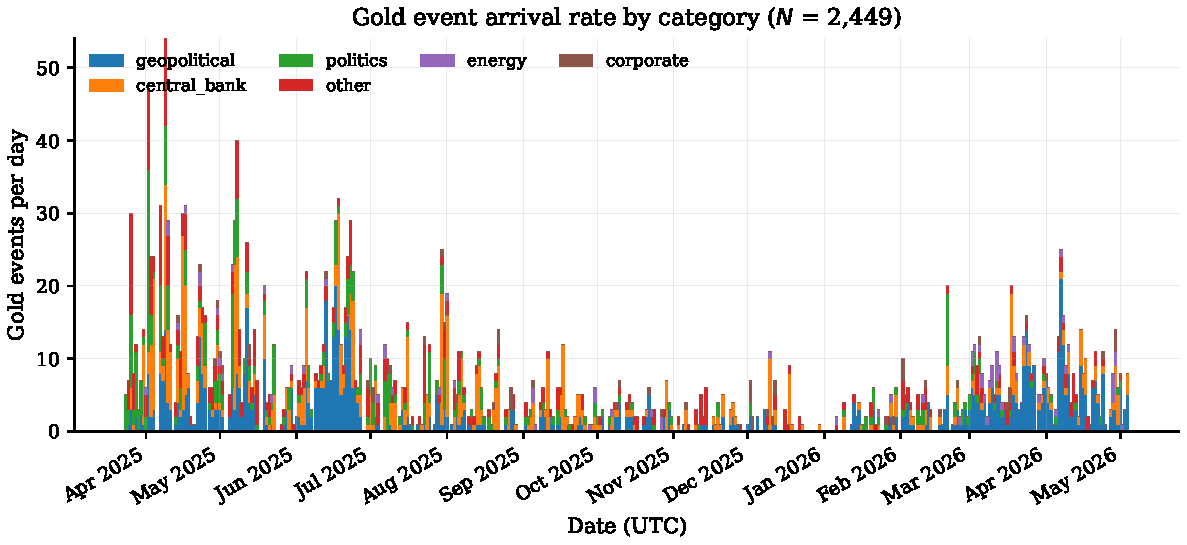
\includegraphics[width=\textwidth]{figures/figure_2_event_timeline.pdf}
\caption{Daily arrival rate of gold news events by category, with
the publisher's \texttt{\$MACRO} tag excluded. The horizontal axis
spans the thirteen-month sample window. Stack ordering follows the
overall category volume.}
\label{fig:event-timeline}
\end{figure}

Table~\ref{tab:sentiment-dist} reports the distribution of the
three sentiment classifiers (the LLM, the Loughran-McDonald
dictionary, and FinBERT-tone) across the full event sample,
together with pairwise label agreement. The three classifiers
disagree substantially: pairwise USD agreement is below $40\%$ for
every pair, and the LLM is the only one of the three that produces
asset-specific labels (USD $\neq$ NDX on $73.5\%$ of events).
Section~\ref{ssec:results-direction} translates these differences
into direction hit rates against realised price moves.

\begin{table}[!htbp]
\centering
\caption{Sentiment label distribution and pairwise classifier agreement.}
\label{tab:sentiment-dist}
\begin{threeparttable}
\small
\begin{tabular}{lrrrr}
\toprule
\textbf{Classifier} & \textbf{Bull} & \textbf{Bear} & \textbf{Neutral} & \textbf{Total} \\
\midrule
LLM (USD) & 958 (39.1\%) & 845 (34.5\%) & 646 (26.4\%) & 2,449 \\
LLM (NDX) & 817 (33.4\%) & 1,138 (46.5\%) & 494 (20.2\%) & 2,449 \\
Loughran-McDonald & 226 (9.2\%) & 1,052 (43.0\%) & 1,171 (47.8\%) & 2,449 \\
FinBERT-tone & 267 (10.9\%) & 393 (16.0\%) & 1,789 (73.1\%) & 2,449 \\
\midrule
\multicolumn{5}{l}{\textit{Pairwise label agreement on USD sentiment ($N$=2,449)}} \\
\quad LLM USD vs LM & \multicolumn{4}{l}{33.0\%} \\
\quad LLM USD vs FinBERT & \multicolumn{4}{l}{28.5\%} \\
\quad LM vs FinBERT & \multicolumn{4}{l}{54.7\%} \\
\midrule
\multicolumn{5}{l}{\textit{Cross-asset disagreement (\texttt{sentiment\_usd} $\neq$ \texttt{sentiment\_ndx})}} \\
\quad LLM & \multicolumn{4}{l}{73.5\%} \\
\quad LM, FinBERT & \multicolumn{4}{l}{$0\%$ by construction (single-polarity classifiers)} \\
\bottomrule
\end{tabular}
\begin{tablenotes}
\footnotesize
\item \textit{Notes.} Distribution of discrete sentiment labels
across the full event sample for each classifier, with column
percentages in parentheses. LM and FinBERT produce a single
polarity per event and therefore cannot disagree across
assets. Pairwise agreement reports the share of events on
which the two classifiers assign the same USD label.
\end{tablenotes}
\end{threeparttable}
\end{table}

